\documentclass[amsmath,amssymb,twocolumn,superscriptaddress]{revtex4-1}

\usepackage{graphicx}% Include figure files
\usepackage{dcolumn}% Align table columns on decimal point
\usepackage{bm}% bold math
\usepackage[detect-all]{siunitx}
\usepackage{hyperref}% add hypertext capabilities
\usepackage{xr}

\begin{document}                  % DO NOT DELETE THIS LINE

\title{An Introduction to Classical Molecular Dynamics Simulation for Experimental Scattering Users}

\author{A.~R. McCluskey}
\email{a.r.mccluskey@bath.ac.uk}
\email{andrew.mccluskey@diamond.ac.uk}
\affiliation{Department of Chemistry, University of Bath, Claverton Down,
Bath, BA2 7AY, UK}
\affiliation{Diamond Light Source, Harwell Campus, Didcot, OX11 0DE, UK}

\author{J. Grant}
\affiliation{Computing Services, University of Bath, Claverton Down, Bath, BA2 7AY, UK}

\author{A.~R. Symington}
\affiliation{Department of Chemistry, University of Bath, Claverton Down,
Bath, BA2 7AY, UK}

\author{T.~Snow}
\affiliation{Diamond Light Source, Harwell Campus, Didcot, OX11 0DE, UK}
\affiliation{School of Chemistry, University of Bristol, Bristol, BS8 1TS, UK}

\author{J.~Doutch}
\affiliation{ISIS Facility, Rutherford Appleton Laboratory, STFC, Chilton, Didcot, OX11 0QX, UK}

\author{B.~J. Morgan}
\email{b.j.morgan@bath.ac.uk}
\affiliation{Department of Chemistry, University of Bath, Claverton Down,
Bath, BA2 7AY, UK}

\author{S.~C. Parker}
\affiliation{Department of Chemistry, University of Bath, Claverton Down,
Bath, BA2 7AY, UK}

\author{K.~J. Edler}
\affiliation{Department of Chemistry, University of Bath, Claverton Down,
Bath, BA2 7AY, UK}

\date{\today}

\begin{abstract}
\noindent Classical molecular dynamics simulations are a common component of multi-modal analyses from scattering measurements, such as small-angle scattering and diffraction.
Users of these experimental techniques often have no formal training in the theory and practice of molecular dynamics simulation, leading to the possibility of these simulations being treated as a ``black box'' analysis technique.
In this article we describe an open educational resource (OER) designed to introduce classical molecular dynamics to users of scattering methods.
This resource is available as a series of interactive web pages, which can be easily accessed by students, and as a open source software repository, which can be copied, modified, and redistributed by educators.
The topic covered in this OER include classical atomistic modelling, parameterising interatomic potentials, molecular dynamics simulations, typical sources of error, and some of the approaches to using simulations in the analysis of scattering data.
\end{abstract}

\maketitle                        % DO NOT DELETE THIS LINE

\section{Introduction}

\noindent The use of molecular dynamics simulations to help analyse and interpret experimental data from small-angle scattering and diffraction studies has grown significantly over the past ten years \cite{pan_molecular_2012,boldon_review_2015,hub_interpreting_2018,ivanovic_temperature-dependent_2018,east_structural_2016,wall_conformational_2014,wall_internal_2018,satoh_multiple_2015},
with the percentage of small-angle scattering publications that mention molecular dynamics reaching more than \SI{20}{\percent} in 2018 (Fig.~\ref{fig:growth}).
Users of scattering and diffraction techniques often have backgrounds in experimental science, and may have received little formal training in the theory or practice of computational modelling.
This can lead to molecular dynamics simulations being used as a ``black box'', without understanding the underlying methodologies, or considering possible sources of error.
The use of molecular simulations without any technical understanding can lead to unintended but severe errors.
To help support researchers use molecular dynamics simulation in their analysis of scattering data, while reducing this risk of modelling errors, a number of software tools, such as WAXSiS and SASSIE \cite{chen_validating_2014,knight_waxsis_2015,perkins_atomistic_2016}, have been developed that present easy-to-use, graphical, web-based user interfaces.

A complementary approach is to organise educational activities, such as lectures or workshops, tailored to introduce molecular simulation techniques to audiences of scattering and diffraction users.
One example is the annual ISIS Neutron Training Course, which includes a module titled ``An Introduction to Molecular Dynamics for Neutron Scattering''.
This module covers the fundamentals of classical molecular dynamics simulation, presents applications of these methods in neutron science, and gives students practical hands-on experience with the SASSIE software package \cite{perkins_atomistic_2016}.

%
\begin{figure}
\label{fig:growth}
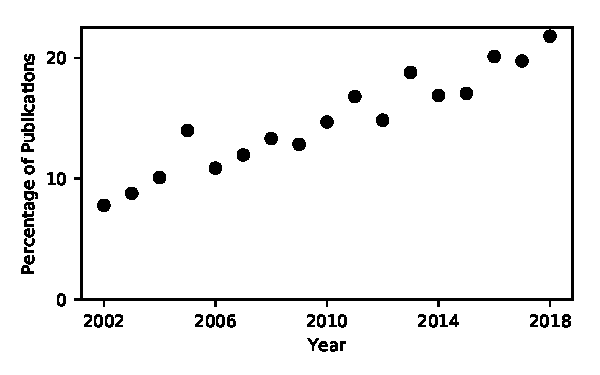
\includegraphics[width=0.48\textwidth]{figures/chem_data_py.pdf}
\caption{The annual percentage of publications that mention ``small angle scattering'' that also mention ``molecular dynamics'', determined from the numbers of matching Google Scholar results.}
\end{figure}
%

While lectures and workshops are an effective tool for education and training, participation can be limited due to difficulties attending in person (due to location or cost) or physical limits on student numbers.
An alternative educational strategy  gaining popularity within scientific and engineering communities is the publication of technology-enhanced open educational resources (OERs).
These are courses, lectures, or learning resources published online that are freely available for use by anyone. In addition to their broad accessibility, these resources have permissive ``open'' copyright licences that allow their use in the ``5R activities'': retain, reuse, revise, remix, and redistribute \cite{wiley_open_2018}.
Publishing a resouce as an OER increases its reach and impact, because others may use it in their own teaching not only in its original form, but are free to modify, and redistribute, the material to better suit their aims.
The Jupyter Notebook framework \cite{kluyver_jupyter_2016} has become a popular platform for OERs that teach computational skills, because it allows authors to include instructional text, images, and other media, alongside executable editable code, in an example of ``literate programming'' \cite{knuth_literate_1984}.
This format encourages students to directly interact with code examples by running, editing, and rerunning these within the source document \cite{barba_cybertraining_2017}, supporting exploratory experiential learning \cite{Papert_Mindstorms1993}.

Here, we present an online, open-source, interactive learning resource written to introduce members of the scattering and diffraction community to molecular dynamics simulations.
This OER comprises six lessons that introduce classical molecular dynamics methods, and show how these can be used in the context of scattering [can this be more specific?] in a multi-modal analysis.
We use the open-source Python library pylj \cite{mccluskey_pylj_2018} to provide simple, but computationally authentic, examples of simulations, that demonstrate visually and programmatically the conceptual relationships between simulation and scattering techniques.
In this article, we discuss the structure of the resource and describe how a student may get the most from the resource \footnote{In this work \emph{the student} refers to anyone working through the OER, regardless of career position.}.

\section{Assumed prior knowledge}

The OER, entitled \emph{``The Interaction Between Simulation and Scattering''} makes use of the Python programming language to include interactive examples of mathematical and algorithmic content.
To be able to fully use this resource, therefore, requires some knowledge of, or willingness to learn, Python.
We have, however, attempted to design the resource in such a fashion that an in-depth knowledge of Python is not a prerequisite.
It is anticipated that the users of this resource have some experience of at least undergraduate level chemistry or physics, and a commensurate level of mathematical understanding.
This background knowledge will be particularly important for the sections dealing with the functional form and chemical basis of classical interaction potentials.

\section{Resource construction}

The resource is currently available online, at \url{http://pythoninchemistry.org/sim_and_scat}.
These webpages were written as a series of Jupyter Notebooks and Markdown files, which were then compiled using the \texttt{jupyter-book} tool \cite{lau_jupyter/jupyter-book_2019}.
This system allows Python code blocks to be included alongside the textual content, providing algorithmic details whilst also facilitating interactivity, though both Thebelab and BinderHub integrations \cite{ragan-kelley_minrk/thebelab_2019,ragan-kelley_jupyterhub/binderhub_2019,jupyter_binder_2018}.
Interacting with the resource in this fashion will aloow the student to either run the Python code directly in the resource interface (Thebelab), or easily launch a MyBinder window to more intensive visualisations (such as pylj).
We believe that the interactive nature of the resource will facilitate understanding allowing the students to gain more than would be obtained from a traditional lecture or handout material \cite{knuth_literate_1984}.

The resource is provided under a CC-BY-SA-4.0 license \cite{noauthor_creative_2019} and builds on the growing library of open educational resources.
The open-source nature of this license means that anyone may use the material to enhance their own educational platform and experts in the field may contribute to improving the resource.
The source code for the resource is available at \url{https://github.com/pythoninchemistry/sim_and_scat} \cite{mccluskey_pythoninchemistry/sim_and_scat_2019}.

\section{Resource outline}

The resource follows a simple outline to introduce important aspects of molecular dynamics simulations.
Code blocks are used to gradually build up the student's understanding of the various concepts.

\subsection{Home}

The welcome page introduces the resource and gives the student information about how the resource may be used, including details of Thebelab and BinderHub integration.
Furthermore, this page gives information about the use and sharing of the content of the resource including details of the license.
This page also includes an authors and contributors list.

\subsection{Classical methods}

Following the introduction, concepts relating broadly to classical simulation methods are introduced.
This includes the functional nature of potential modelling and gives some examples, such as the Lennard-Jones and Buckingham potential models \cite{lennard-jones_determination_1924,buckingham_classical_1938}.
The potential model parameterisation is briefly covered including the use of higher accuracy quantum mechanical calculations to do so.
The presence of off-the-shelf, general potential models are discussed; with particular attention paid to the caveat that they may still require system specific optimisations.
Finally, we mention mixing rules; again discussing the possible problems that a user may encounter related to system specificity.

\subsection{Molecular dynamics}

Building on the classical potential model methods the student is then presented with molecular dynamics.
This is shown by using different aspects for the method to gradually build up a one-dimensional molecular dynamics simulation using NVE (Number, Volume and Energy) ensembles, the Velocity-Verlet algorithm and the Lennard-Jones potential model \cite{swope_computer_1982,lennard-jones_determination_1924}.
This is introduced in terms of Newton's laws of motion and the generalised equations of motion, which should be familiar to most students.
Finally, different importance considerations for molecular dynamics simulations are described including ensembles, the potential cut-off, and periodic boundary conditions.

\subsection{\texttt{pylj} and the interaction with scattering}

The final aspect of the resource is to utilise a molecular dynamics simulation to understand some scattering profiles.
This is achieved using the open-source \texttt{pylj} package \cite{mccluskey_pylj_2018}, which allows for a two-dimensional simulation or argon particles, interacting through a Lennard-Jones potential, to be performed.
The student is first shown a working \texttt{pylj} simulation and invited to interact with the simulation and the custom plotting functionality of \texttt{pylj}.
In the final lessons, a formulation of the Debye equation \cite{debye_zerstreuung_1915} is given and the student is invited to observe the effect of simulation temperature on the resulting scattering profile.
There is mention of other, faster, algorithms for the determination of scattering profiles, such as the Fibonacci sequence or Golden Vectors methods \cite{svergun_solution_1994,watson_rapid_2013}.

\section{Future outlook}

In the future, we hope that the nature of the material, as an OER, will promote interest from other parties towards reuse, and remixing the material.
Furthermore, we hope to implement this material within training at the ISIS Neutron and Muon Source as well as Diamond Light Source.
Finally, it is hoped, \textit{via} student and community feedback, that the improvement of implementation, materials, and general pedagogy of the resource can be achieved, driving up the quality and depth of molecular dynamics analyses performed on results obtained from scattering and diffraction measurements.

\section{Author contributions}

The open education resource was developed, and the manuscript written, by A. R. M. with input from all authors.

\begin{acknowledgements}
A. R. M. is grateful to the University of Bath and Diamond Light Source for co-funding a studentship (Studentship No. STU0149).
B. J. M. acknowledges support from the Royal Society (Grant No. UF130329).
\end{acknowledgements}

\bibliography{bib.bib}


\end{document}                    % DO NOT DELETE THIS LINE
